\documentclass[../hw.tex]{subfiles}

\begin{document}
\setcounter{section}{12}
\begin{center}
  \section*{Homework 12} \label{sec:homework12}
\end{center}
\addcontentsline{toc}{section}{\nameref{sec:homework12}}
\hrule \vspace{10px}
\paragraph*{1.} (a) The canonical momenta are
\begin{align*}
    p_r &= \pdv{\lagr}{\dot{r}} = m \dot r \\
    p_\theta &= \pdv{\lagr}{\dot{\theta}} = m r^2 \dot \theta \\
    p_\phi &= \pdv{\lagr}{\dot{\phi}} = m r^2 \sin^2 \theta \dot \phi
\end{align*}
(b) So the Hamiltonian is
\begin{align*}
    \mathcal{H} &= \sum_i p_i \dot q_i - \lagr \\
    &= p_r \dot r + p_\theta \dot \theta + p_\phi \dot \phi
         - \frac{1}{2}m \qt(\dot r^2 + r^2 \dot \theta^2 + r^2 \sin^2 \theta \dot \phi^2) + U
\end{align*}
and substituting
\begin{align*}
    \dot r &= \frac{p_r}{m}, \quad \dot \theta = \frac{p_\theta}{m r^2}, 
    \quad \dot \phi = \frac{p_\phi}{m r^2 \sin^2 \theta}
\end{align*}
we get
\begin{align*}
    \mathcal{H} &= \frac{1}{m} \qt(p_r^2 + \frac{p_\theta^2}{r^2} 
        + \frac{p_\phi^2}{r^2 \sin^2\theta}) 
        - \frac{1}{2m} \qt(p_r^2 + \frac{p_\theta^2}{r^2} + \frac{p_\phi^2}{r^2 \sin^2\theta}) + U \\
    &= \frac{1}{2m} \qt(p_r^2 + \frac{p_\theta^2}{r^2} + \frac{p_\phi^2}{r^2 \sin^2\theta}) + U(r, \theta, \phi)
\end{align*}
Finally, the three sets of Hamilton's equations are
\newcommand{\ham}{\mathcal{H}}
\begin{align*}
    \dot r &= \pdv{\ham}{p_r} = \frac{p_r}{m} \\ 
    \dot p_r &= -\pdv{\ham}{r} = \frac{1}{mr^3} \qt(p_\theta^2 + \frac{p_\phi^2}{\sin^2\theta}) - \pdv{U}{r} \\
    \dot \theta &= \pdv{\ham}{p_\theta} = \frac{p_\theta}{m r^2} \\
    \dot p_\theta &= -\pdv{\ham}{\theta} = \frac{1}{mr^2}\qt(\frac{p_\phi^2 \cos\theta}{\sin^3\theta}) - \pdv{U}{\theta} \\
    \dot \phi &= \pdv{\ham}{p_\phi} = \frac{p_\phi}{m r^2 \sin^2\theta} \\
    \dot p_\phi &= -\pdv{\ham}{\phi} = -\pdv{U}{\phi}
\end{align*}
\newpage
\paragraph*{2.} (a) The coordinates of the spinning pendulum is 
\begin{align*}
    r = L, \quad \phi = \omega t 
\end{align*}
where the azimithal component is time-dependent, and the polar coordinate is found by the EL equation
\begin{align*}
    \dv{t} \pdv{\lagr}{\dot \theta} - \pdv{\lagr}{\theta} = 0 \\
    \implies \ddot \theta = \omega^2 \sin \theta \cos \theta - \frac{g}{L} \sin \theta 
\end{align*}
which is also time-dependent. (b) The canonical momenta are
\begin{align*}
    p_r &= \pdv{\lagr}{\dot r} = 0 \\
    p_\theta &= \pdv{\lagr}{\dot \theta} = m L^2 \dot \theta \\
    p_\phi &= \pdv{\lagr}{\dot \phi} = 0
\end{align*}
and the Hamiltonian is
\begin{align*}
    \ham &= \sum_i p_i \dot q_i - \lagr \\
    &= p_\theta \dot \theta - \lagr \\
    &= m L^2 \dot \theta^2 
        - \frac{1}{2} m L^2 \qt(\dot \theta^2 + \omega^2 \sin^2 \theta) 
        + m g L(1 - \cos \theta) \\
    &= \frac{1}{2} m L^2 \qt(\dot \theta^2 - \omega^2 \sin^2 \theta) + m g L(1 - \cos \theta) \\
    &\neq T + U
\end{align*}
(c)
\begin{align*}
    \ham &= T' - \frac{1}{2} mL^2 \omega^2 \sin^2\theta + m g L(1 - \cos\theta) \\
    \implies U' &= -\frac{1}{2} mL^2 \omega^2 \sin^2\theta + m g L(1 - \cos\theta)
\end{align*}
Finding the minimum of $U'$, we have
\begin{align*}
    \pdv{U'}{\theta} = 0 = -mL^2 \omega^2 \sin\theta \cos\theta + mgL \sin\theta \\
    0 = -L \omega^2 \cos\theta + g 
    \implies \theta = \arccos \frac{g}{L \omega^2}
\end{align*}
so theta is not always zero. Plotting $U'$, we have a mexican hat cross section:
\begin{figure}[ht]
    \centering
    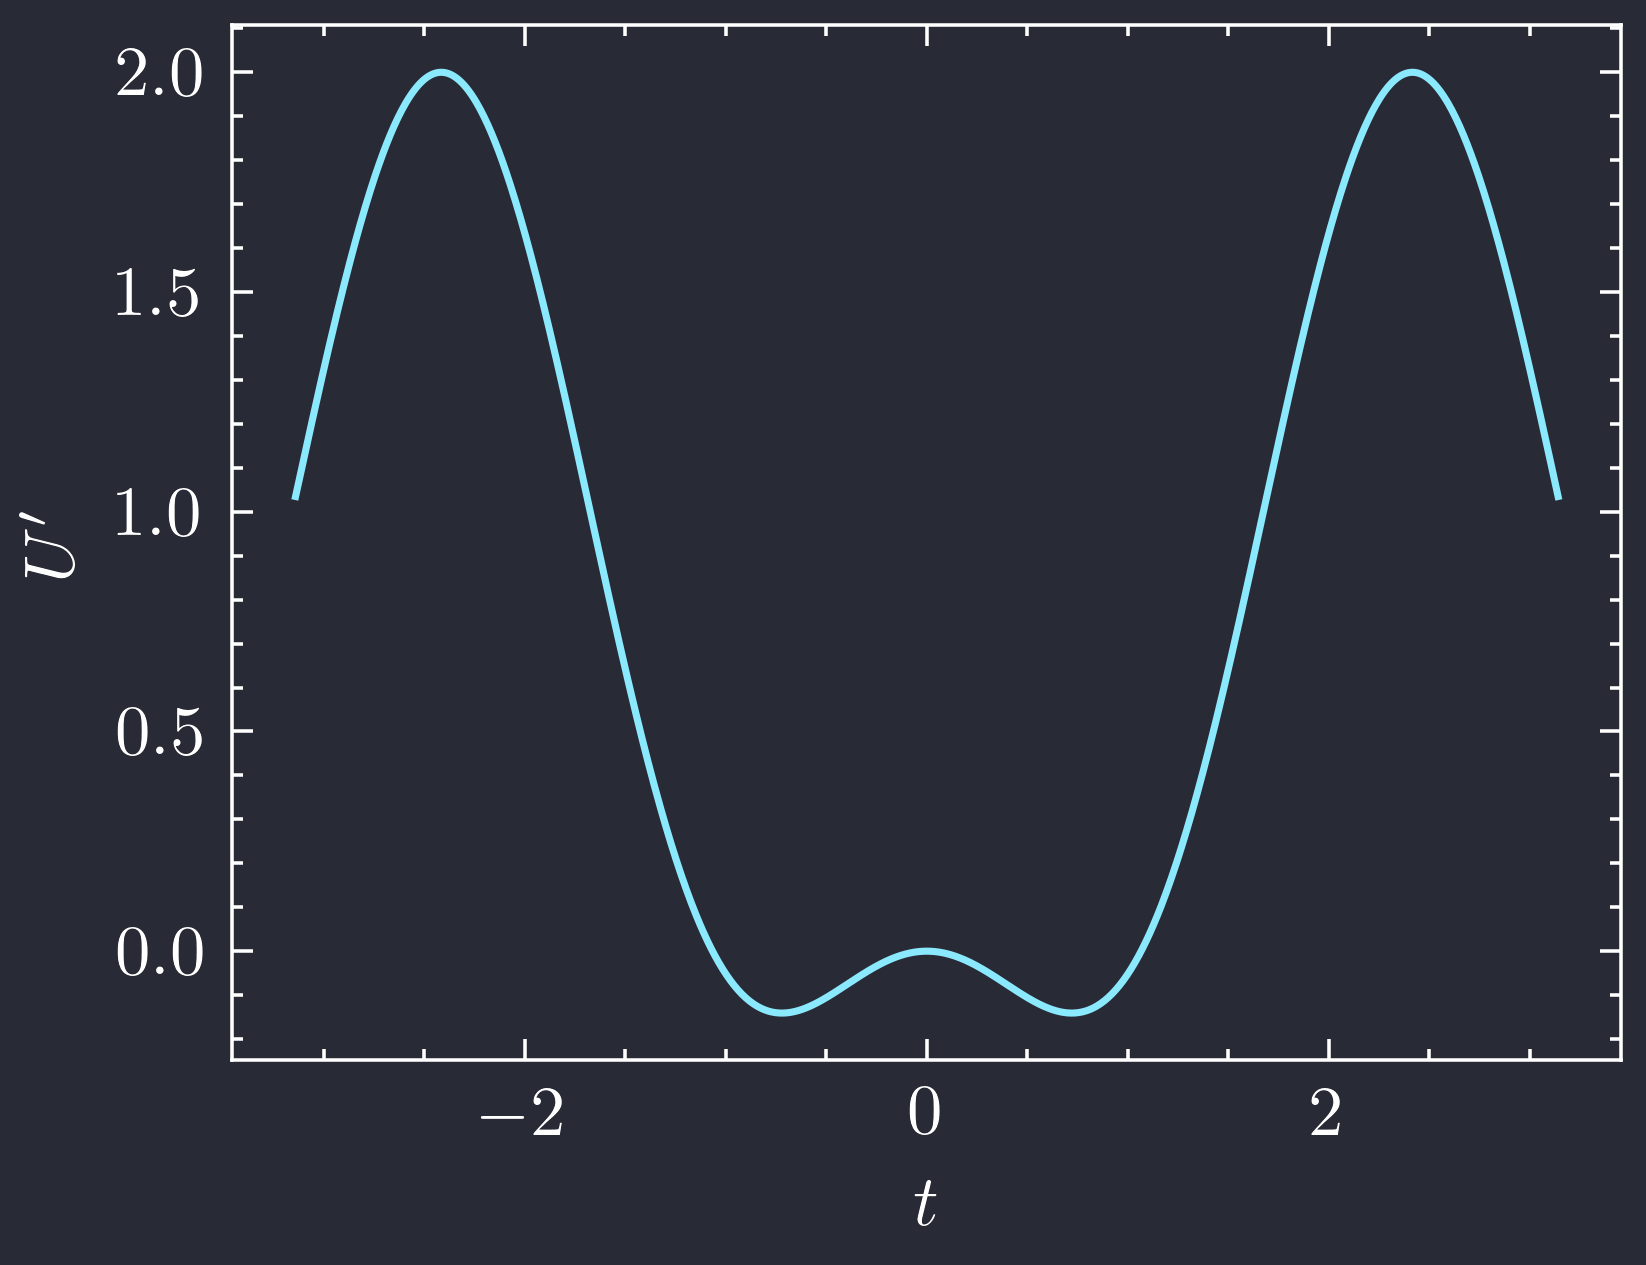
\includegraphics[width=0.3\textwidth]{hw12.png}
    \caption{Plot of $U'$ where $L = g = m = 1$ and $\omega^2 = 1.3^2 > g/L$}
\end{figure}

\newpage
\paragraph*{3.} (a) Hamilton's equations for the particle:
\begin{align*}
    \dot x &= \pdv{\ham}{p_x} = \qt[\frac{mc^2}{\sqrt{1 + (\vb p/mc)^2}}\frac{1}{2} 2(\vb p /mc) \frac{1}{mc}]_x
    = \frac{p_x}{m\sqrt{1 + (p_x/mc)^2}} \\
    \dot{p}_x &= -\pdv{\ham}{x} = -\pdv{U}{x}
\end{align*}
and similarly for $y$ and $z$. (b) For small $\vb p/mc$, $\sqrt{1 + (\vb p/mc)^2} \approx 1$ so
\begin{align*}
    \dot x = \frac{p_x}{m} = \frac{m v_x}{m} = v_x
\end{align*}
which reduces to the Newtonian case.

\paragraph*{4.} (a) The canonical momenta are
\begin{align*}
    \vb p &= \pdv{\lagr}{\dot{\vb r}} = m \dot{\vb r} 
        + q \vb A
\end{align*}
And the Hamiltonian is
\begin{align*}
    \ham &= \vb p \cdot \dot{\vb r} - \lagr \\
    &= m \dot{\vb r} \cdot \dot{\vb r} + q \vb A \cdot \dot{\vb r} 
        - \frac{1}{2} m \dot{\vb r}^2 + q (\phi_e - \dot{\vb r} \cdot \vb A) \\
    &= \frac{1}{2} m \dot{\vb r}^2 + q \phi_e
\end{align*}
or using $\dot{\vb r} = \frac{1}{m} (\vb p - q \vb A)$,
\begin{align*}
    \ham &= \frac{1}{2m}(\vb p - q \vb A)^2 + q \phi_e
\end{align*}
(b) Using Hamilton's equation:
\begin{align*}
    \dot{\vb r} &= \pdv{\ham}{\vb p} = \frac{1}{m} (\vb p - q \vb A) = \vb v
\end{align*}
and taking the derivative gives,
\begin{align*}
    m \ddot{\vb r} &= \dot{\vb p} - q \dv{\vb A}{t}
\end{align*}
where
\begin{align*}
    \dv{\vb A}{t} &= \pdv{\vb A}{t} + \pdv{\vb A}{x}\dv{x}{t} + \pdv{\vb A}{y}\dv{y}{t} + \pdv{\vb A}{z}\dv{z}{t} \\
    &= \pdv{\vb A}{t} + (\vb v \cdot \grad) \vb A
\end{align*}
To find the first term, we use the second part of Hamilton's equation:
\begin{align*}
    \dot{p}_x &= - \pdv{\ham}{x} \\
    &= \frac{q}{m} (\vb p - q \vb A) \pdv{\vb A}{x} - q \pdv{\phi_e}{x}\\
    &= q \vb v \pdv{\vb A}{x} - q \pdv{\phi_e}{x}
\end{align*}
so 
\begin{align*}
    \dot{\vb p} &= q \grad(\vb v \cdot \vb A) - q \grad \phi_e
\end{align*}
This gives us
\begin{align*}
    m \ddot{\vb r} &= q[\grad(\vb v \cdot \vb A) - \grad \phi_e - \pdv{\vb A}{t} - (\vb v \cdot \grad) \vb A] \\
    &= q[\vb E + \grad(\vb v \cdot \vb A) - (\vb v \cdot \grad) \vb A]
\end{align*}
where we can use the B(AC)-C(AB) rule to simplify
\begin{align*}
    \vb v \cross (\curl \vb A) &= \grad(\vb v \cdot \vb A) - (\vb v \cdot \grad) \vb A
\end{align*}
so
\begin{align*}
    m \ddot{\vb r} &= q[\vb E + \vb v \cross (\curl \vb A)] \\
    &= q(\vb E + \vb v \cross \vb B)
\end{align*}

\paragraph*{5.} The components of the angular momentum are
\begin{align*}
    \vb r \cross \vb p &= \mqty| \vu x & \vu y & \vu z \\ x & y & z \\ p_x & p_y & p_z | \\
\end{align*}
so
\begin{align*}
    \ell_x &= y p_z - z p_y \\
    \ell_y &= z p_x - x p_z \\
    \ell_z &= x p_y - y p_x
\end{align*}
Poisson brakets of angular momenta:
\begin{align*}
    [\ell_x, \ell_y] &= 
    \sum_i \qt(\pdv{\ell_x}{r_i} \pdv{\ell_y}{p_i} - \pdv{\ell_y}{r_i} \pdv{\ell_x}{p_i}) \\
    &= \qt(\pdv{\ell_x}{x} \pdv{\ell_y}{p_x} - \pdv{\ell_y}{x} \pdv{\ell_x}{p_x})
        + \qt(\pdv{\ell_x}{y} \pdv{\ell_y}{p_y} - \pdv{\ell_y}{y} \pdv{\ell_x}{p_y})
        + \qt(\pdv{\ell_x}{z} \pdv{\ell_y}{p_z} - \pdv{\ell_y}{z} \pdv{\ell_x}{p_z}) \\
    &= 0 + 0 + [(-p_y)(-x) - (p_x)(y)] \\
    &= x p_y - y p_x = \ell_z
\end{align*}
and similarly for the other components:
\begin{align*}
    [\ell_y, \ell_z] &= \qt(\pdv{\ell_y}{x} \pdv{\ell_z}{p_x} - \pdv{\ell_z}{x} \pdv{\ell_y}{p_x})
        + \qt(\pdv{\ell_y}{y} \pdv{\ell_z}{p_y} - \pdv{\ell_z}{y} \pdv{\ell_y}{p_y})
        + \qt(\pdv{\ell_y}{z} \pdv{\ell_z}{p_z} - \pdv{\ell_z}{z} \pdv{\ell_y}{p_z}) \\
        &= [(-p_z)(-y) - (p_y)(z)] + 0 + 0 \\
        &= y p_z - z p_y = \ell_x
\end{align*}
there is a pattern here\dots
\begin{align*}
    [\ell_z, \ell_x] &= \qt(\pdv{\ell_z}{y} \pdv{\ell_x}{p_y} - \pdv{\ell_x}{y} \pdv{\ell_z}{p_y}) \\
        &= (-p_x)(-z) - (p_z)(x) \\
        &= z p_x - x p_z = \ell_y
\end{align*}
\end{document}